\section{Introduction}
\label{sec:introduction}

The design of lightweight structures is a crucial aspect in the automotive industry.
In the following, a topology optimization of the hub carrier for an ultra-efficient lightweight battery-electric vehicle is presented.
In particular, the vehicle considered for this work is \textit{Asteria} (see Figure \ref{fig:asteria}), developed by the \textit{Green MECC} team at Politecnico di Milano for the \textit{Shell Eco-marathon} competition.

\begin{figure}[H]
    \centering
    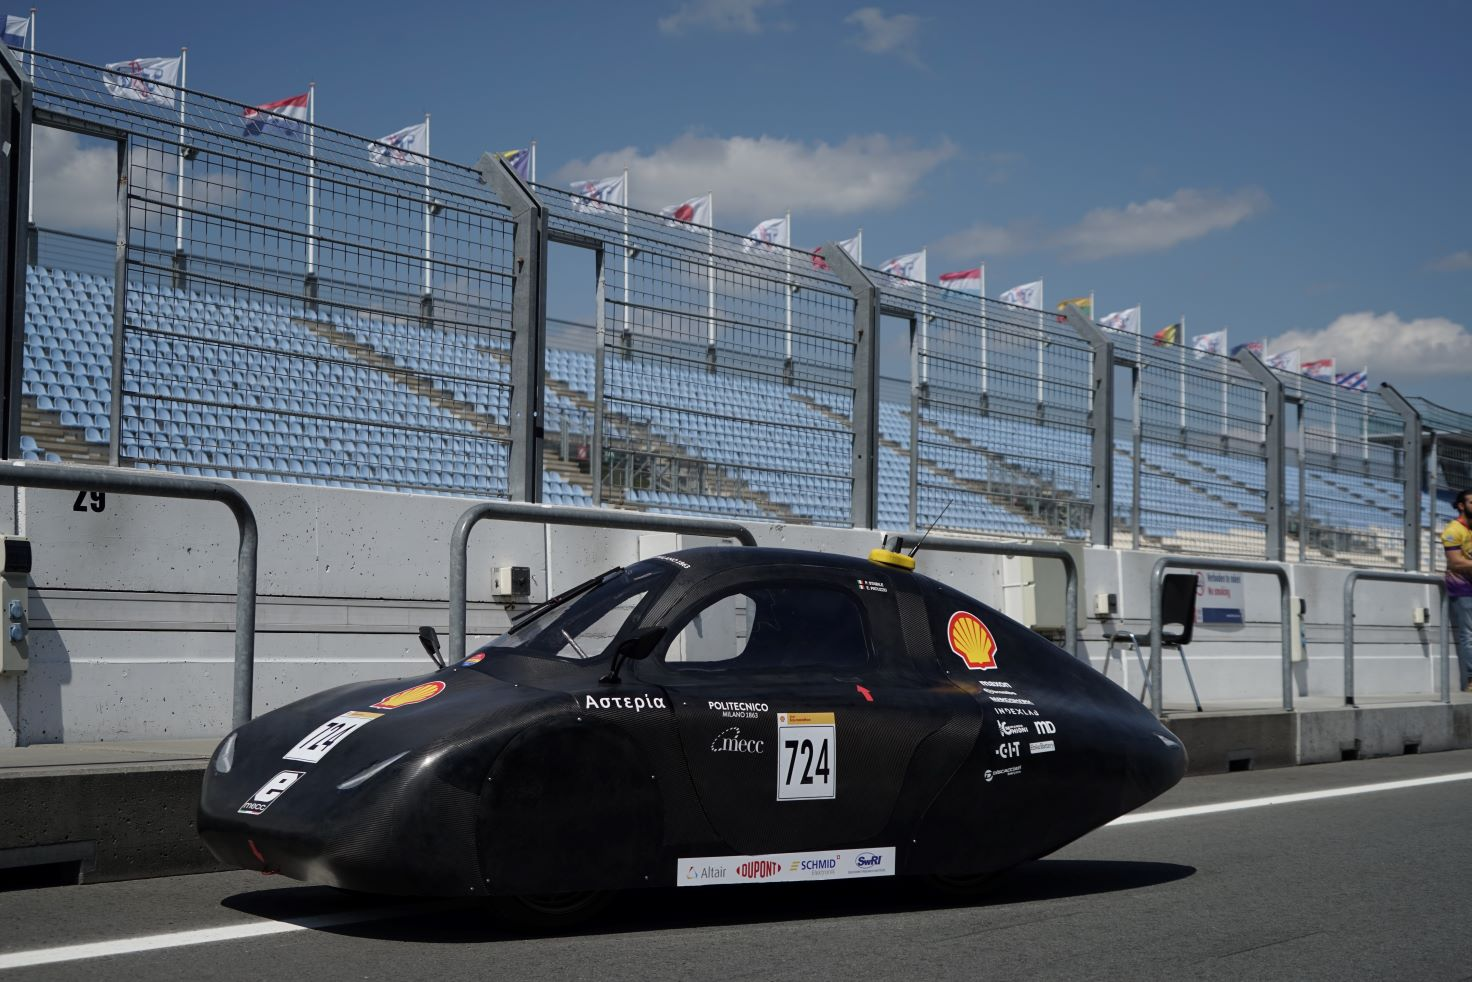
\includegraphics[width=0.7\textwidth]{img/Asteria.jpg}
    \caption{Asteria vehicle \cite{GreenTeamPoliMi}.}
    \label{fig:asteria}
\end{figure}

During motion, the main sources of energy dissipation are mass (inertia), tire rolling resistance, and aerodynamic drag.
Moreover, the vehicle mass has the most significant impact on energy consumption, emphasizing the importance of lightweight design.


\paragraph{Project goals}

The goal of this project is to optimize the hub carrier by maximizing structural stiffness while minimizing mass.
As we will see, different load scenario and constraints are considered to ensure the hub carrier is able to withstand the forces generated during the competition.
Some constraints will also be imposed to ensure the manufacturability of the final design.


\paragraph{Tools}

The optimization process will be carried out using some of the software package provided by the \texttt{Altair HyperWorks} suite \cite{AltairHyperworks}.
In particular, we opted for the following tools:

\begin{itemize}
    \item \texttt{HyperMesh}: preprocessing and meshing phase;
    \item \texttt{OptiStruct}: topology optimization;
    \item \texttt{HyperView}: post-processing and visualization.
\end{itemize}

Finally, the smoothing of the optimized geometry is performed using \texttt{Altair Inspire}.